\chapter{实验装置与数据样本}
% \chapter{Experimental Apparatus and Data Samples}

本章介绍本分析使用的实验装置与数据基础。首先概述大型强子对撞机和CMS探测器的关键子系统，随后说明数据样本的采集条件与积分亮度，最后描述蒙特卡罗模拟样本的产生流程。这些实验条件为第4章的事例重建与选择提供了物理基础。

\section{大型强子对撞机}
% \section{The Large Hadron Collider}

% [PENDING]
大型强子对撞机（Large Hadron Collider, LHC）位于欧洲核子研究中心（CERN）日内瓦附近的地下隧道中，主环周长约为 27~km，是高能前沿的质子--质子对撞机~\cite{CMS_JINST_2008}。在 LHC Run~3（2022--2024）期间，对撞机提供质心系能量为 $\sqrt{s}=13.6$~TeV 的质子--质子对撞，并为 CMS、ATLAS、ALICE 和 LHCb 实验提供高能强子束流。本文研究的 $pp \to J/\psi + J/\psi + \phi + X$ 过程在 CMS 对撞点在 Run~3 数据采集期间记录的质子--质子对撞数据中寻找。

% [PENDING]
LHC 的质子束被分为若干束团，标准束团间隔为 25~ns，对应约 40~MHz 的束团交叉频率。

% [PENDING]
LHC 的设计瞬时亮度约为 $2\times10^{34}~\text{cm}^{-2}\text{s}^{-1}$，在 Run~3 期间实际运行瞬时亮度超过设计值。这一高瞬时亮度意味着同一次束团交叉中可能包含多个独立的质子--质子相互作用，即堆叠（pileup）。Run~3 期间的平均堆叠约为每次束团交叉 60 个相互作用，具体取决于运行条件。堆叠会影响顶点分辨、带电径迹关联和低动量缪子的在线选择效率；因此，数据采集条件、触发路径版本和堆叠模拟配置均被视为样本定义的一部分。具体的重建对象定义和离线事例选择在第 4 章讨论。

% [PENDING]
本分析使用的数据来自 2022--2024 年 LHC Run~3 数据采集期间，最终的数据集选择、亮度认证和积分亮度将在分析最终确定后记录。

\begin{figure}
  \centering
  \fbox{\parbox{0.82\linewidth}{\centering
    \vspace{1.8cm}
    \textbf{[待填图：LHC 环和四个主要实验]}\\
    建议来源：公开的 CERN/CMS 示意图，使用前注明来源。
    \vspace{1.8cm}
  }}
  \caption{LHC 及其主要实验的布局示意图。最终图应标明 CMS 对撞点并注明公开图像来源。}
  \label{fig:chap03-lhc-layout-placeholder}
\end{figure}

\section{CMS 探测器}
% \section{The CMS Detector}

% [PENDING]
紧凑缪子螺线管（Compact Muon Solenoid, CMS）探测器是 LHC 上的通用型探测器之一。CMS 探测器全长 21.6~m，直径 14.6~m，总重约 14\,000 吨，采用以束流轴为中心的近似圆柱对称结构。由内向外包括硅径迹探测器、电磁量能器、强子量能器、超导螺线管磁体以及嵌入铁返回轭中的缪子系统。超导螺线管是有史以来建造的最大的螺线管磁体，在内部探测器体积中提供 3.8~T 的轴向磁场，并在铁轭中产生约 2~T 的返回场，使带电粒子轨迹弯曲，从而实现动量测量~\cite{CMS_JINST_2008}。

% [PENDING]
本分析的实验灵敏度主要依赖 CMS 对低动量缪子和带电强子径迹的重建能力。两个 $J/\psi$ 候选态通过缪子衰变道重建，$\phi$ 候选态通过带电强子衰变道重建，因此硅径迹探测器、缪子系统和触发系统是本章重点介绍的探测器组成部分。粒子流算法在 CMS 中综合使用各子探测器信息形成全局事例描述~\cite{CMS_PF_RECO_JINST_2017}；本章仅说明其与实验装置和模拟链的关系，具体重建对象选择保留在后续章节。

\begin{figure}
  \centering
  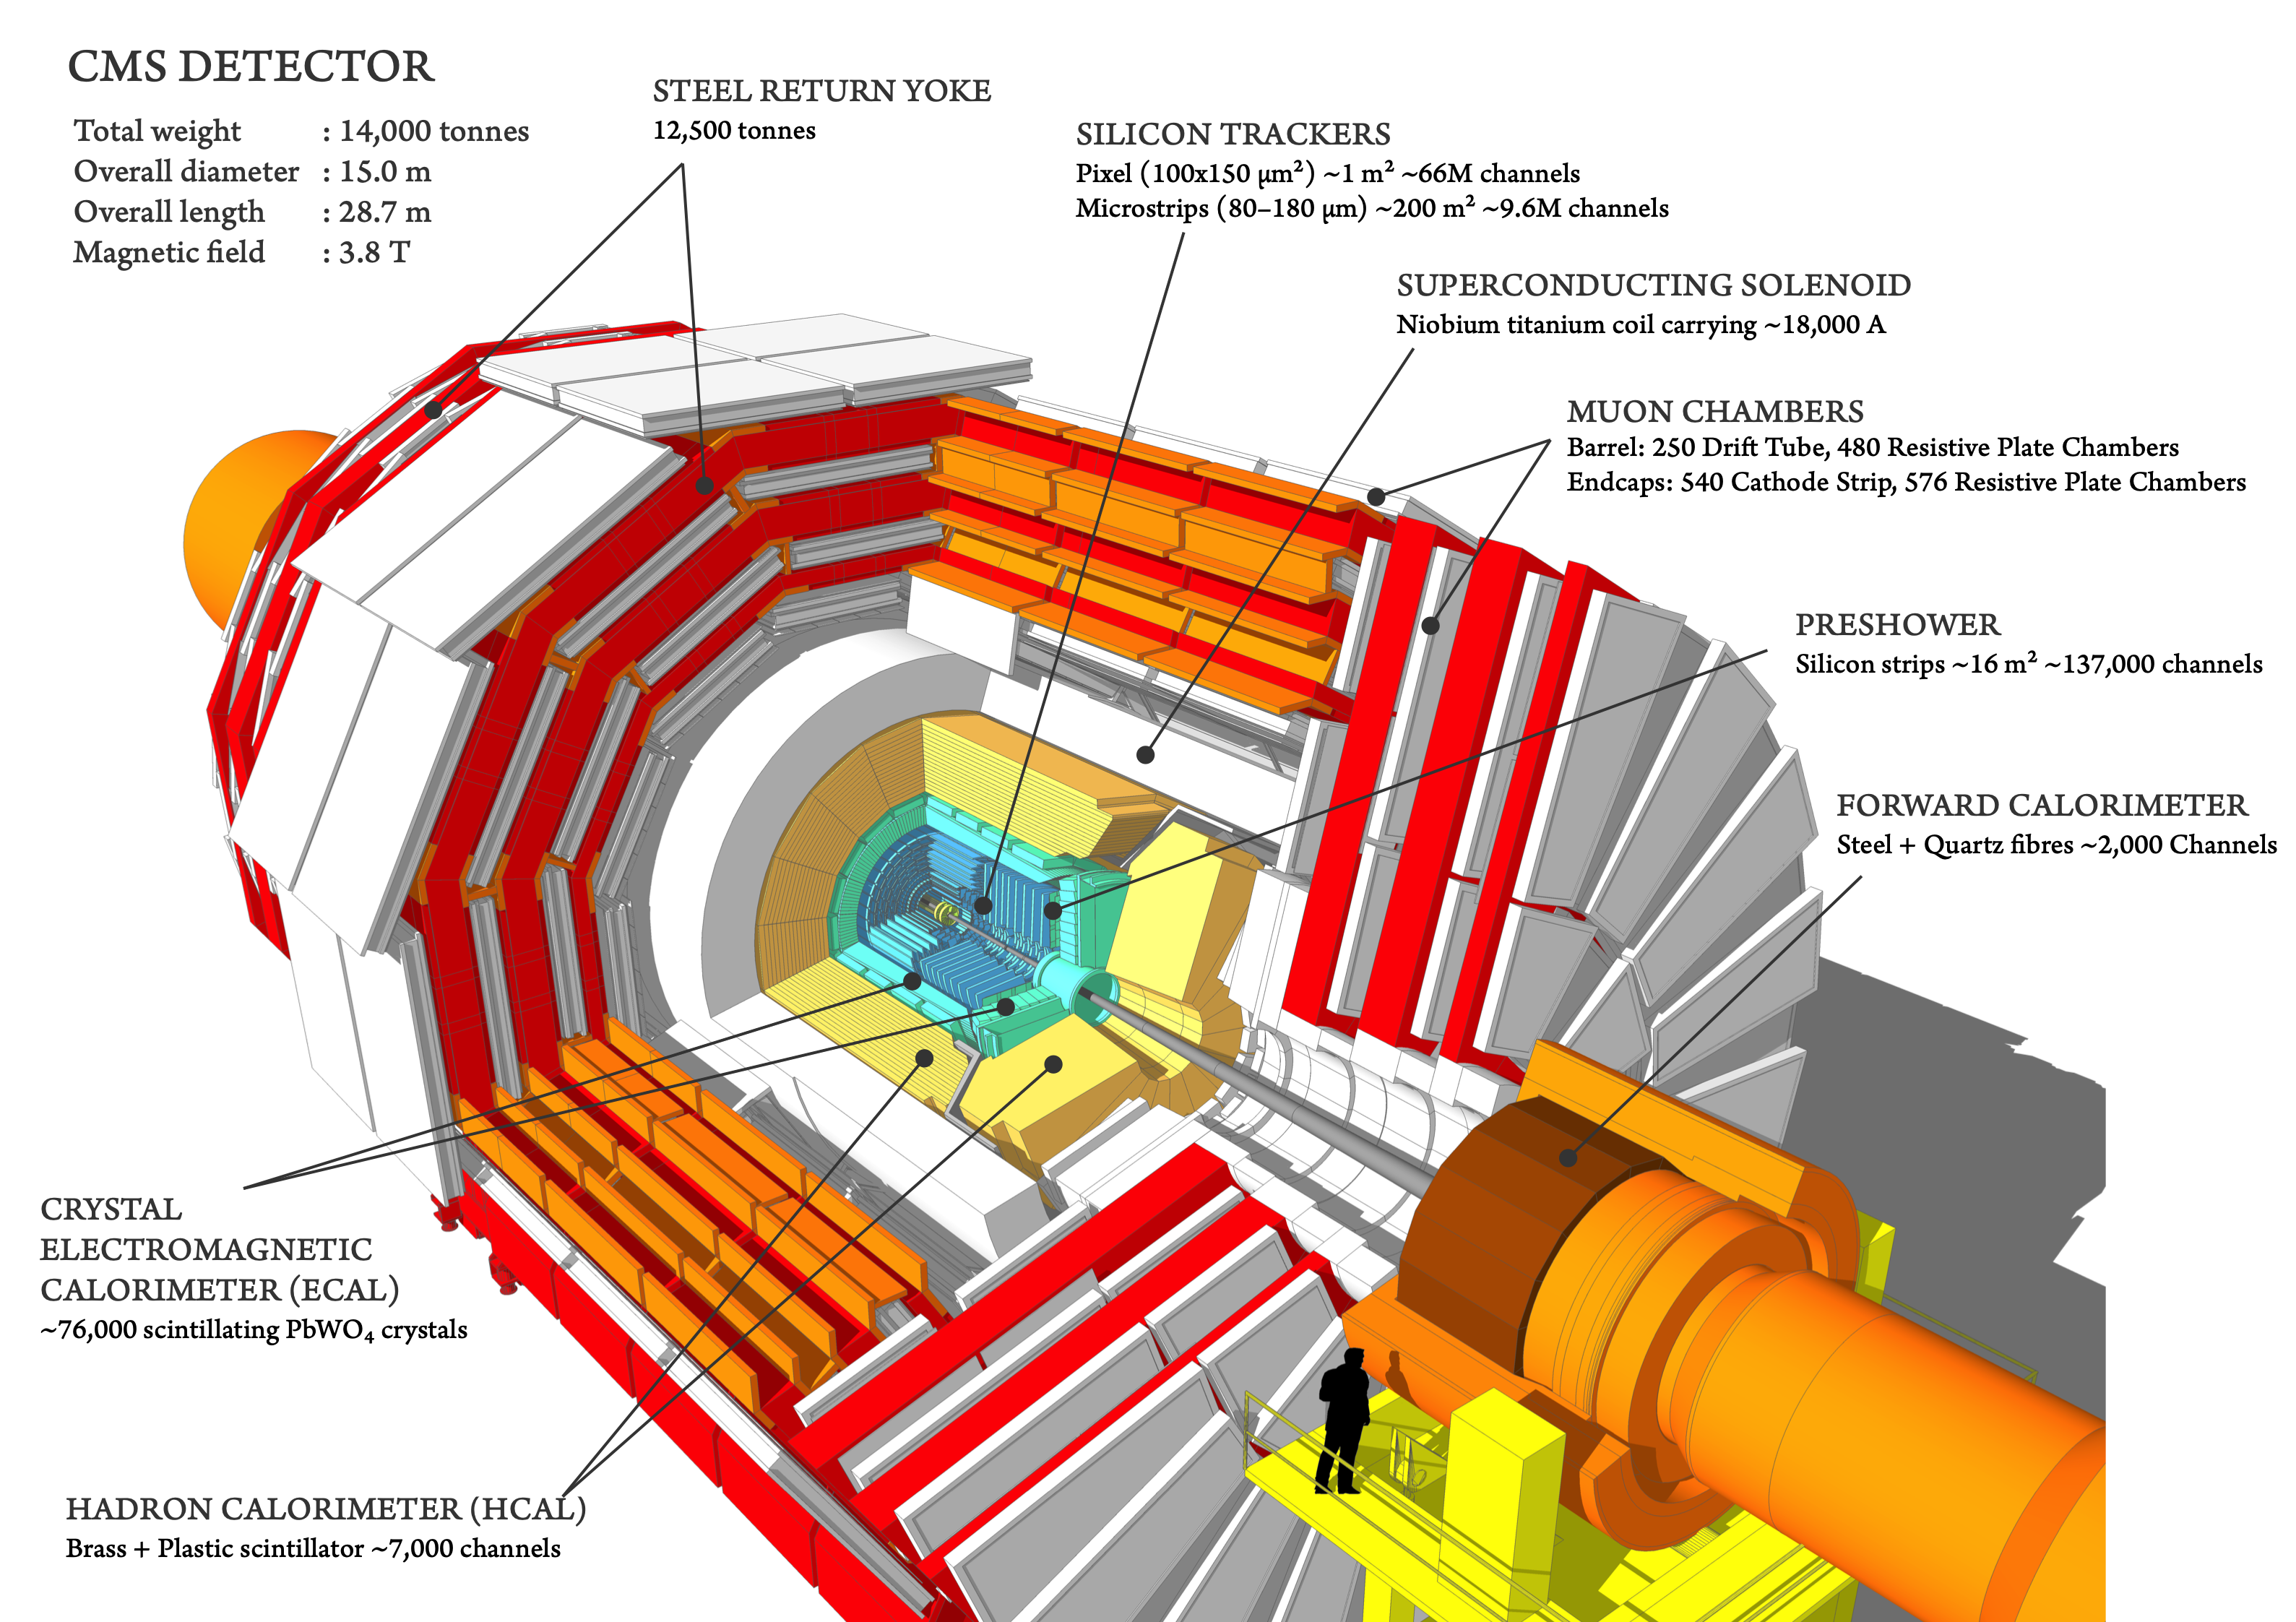
\includegraphics[width=0.85\linewidth]{figures/chap03-experiment-dataset/CMS_disection_Run2.png}
  \caption{CMS 探测器的横向和纵向截面图，展示主要子探测器组件：硅径迹探测器、电磁和强子量能器、超导螺线管磁体以及嵌入铁返回轭中的缪子探测器。\cite{CMS_JINST_2008}。}
  \label{fig:chap03-cms-cutaway}
\end{figure}

\subsection{坐标系与运动学变量}
% \subsection{Coordinate System and Kinematic Variables}

% [PENDING]
CMS 使用右手坐标系，原点位于探测器中心的名义相互作用点。$x$ 轴指向 LHC 环中心，$y$ 轴竖直向上，$z$ 轴沿逆时针束流方向。方位角 $\phi$ 在垂直于束流的平面内定义，极角 $\theta$ 从正 $z$ 轴量起。赝快度定义为 $\eta=-\ln[\tan(\theta/2)]$，横动量定义为 $p_{\mathrm{T}}=p\sin\theta$。两个对象之间的角距离通常写作 $\Delta R=\sqrt{(\Delta\eta)^2+(\Delta\phi)^2}$。

% [PENDING]
在 CMS 对撞点处，束流发光区域（束斑）沿束流方向的典型 RMS 展宽约为数厘米，通过每轮运行中基于径迹的对齐算法进行监测。

\begin{figure}
  \centering
  \fbox{\parbox{0.72\linewidth}{\centering
    \vspace{1.4cm}
    \textbf{[待填图：CMS 坐标系]}\\
    包含 $x$、$y$、$z$、$\theta$、$\phi$、$\eta$ 和横向平面。
    \vspace{1.4cm}
  }}
  \caption{CMS 使用的坐标系和基本运动学变量。}
  \label{fig:chap03-coordinate-placeholder}
\end{figure}

\subsection{硅径迹探测器}
% \subsection{Silicon Tracker}

% [PENDING]
硅径迹探测器位于 CMS 最内层，覆盖 $|\eta|<2.5$ 的区域，由像素探测器和硅微条探测器组成~\cite{CMS_JINST_2008,CMS_TDR_CH6_TRACKING}。像素探测器靠近束流管，提供高精度三维击中信息；硅微条探测器提供更大半径范围内的多层击中信息。

% [PENDING]
像素探测器包含三个桶部层，半径分别为 4、7 和 11~cm，每侧各有两个端盖盘，像素尺寸为 $100 \times 150~\mu\mathrm{m}^2$，在 $r$--$\phi$ 弯曲平面内的空间分辨率约为 10~$\mu$m，在 $z$ 方向约为 20~$\mu$m。

硅微条探测器由约 15\,400 个硅模块组成，总有效面积约 200~m$^2$，分为四个子系统：径迹探测器内桶（TIB，4 层）、径迹探测器外桶（TOB，6 层）、径迹探测器内盘（TID，每侧 3 个小盘，填补 TIB 与 TEC 之间的间隙）和径迹探测器端盖（TEC，每侧 9 个盘，延伸至 $|z| \approx 280$~cm）。内部区域（TIB、TID、最内层 TEC 环）的传感器厚度为 320~$\mu$m，而外部区域（TOB、外层 TEC 环）的传感器厚度为 500~$\mu$m。

一个带电粒子穿过整个径迹探测器通常产生约 13--16 个空间点，其中 3 个由像素探测器提供。在内部径迹接收度范围内，对 $p_{\mathrm{T}} > 1$~GeV 的带电粒子径迹重建效率约为 95\%，误重建率低于百分之几~\cite{CMS_TDR_CH6_TRACKING}。

% [PENDING]
带电粒子的动量通过由这些击中点在 3.8~T 磁场中形成的弯曲轨迹拟合得到。因此，径迹探测器为带电粒子动量测量、相互作用顶点重建和二级顶点定位提供基础输入。

% [PENDING]
在本分析中，硅径迹探测器对 $\phi \to K^+K^-$ 候选态的带电径迹和 $J/\psi \to \mu^+\mu^-$ 衰变中的缪子内径迹均至关重要。径迹质量、顶点拟合和质量约束等分析层面的定义不在本节展开，而在事例重建与选择章节中统一给出。

\subsection{缪子系统}
% \subsection{Muon System}

% [PENDING]
缪子系统位于超导磁体外侧的铁返回轭中，覆盖约 $|\eta|<2.4$ 的区域，采用三种互补的气体探测器技术~\cite{CMS_JINST_2008}。

% [PENDING]
漂移管（Drift Tube, DT）系统覆盖桶部区域（$|\eta| < 1.2$），由沿束流轴排列的五个同心轮上的四个站点（MB1--MB4）组成。内层站点（MB1 和 MB2）的每个腔室包含四个超层，共 12 个灵敏漂移层，而外层站点（MB3 和 MB4）包含三个超层，共 9 层，在 $r$--$\phi$ 弯曲平面内提供约 250~$\mu$m 的单腔室空间分辨率。

阴极条室（Cathode Strip Chamber, CSC）系统覆盖端盖区域（$0.9 < |\eta| < 2.4$），每个端盖有四个站点（ME1--ME4）。每个梯形 CSC 腔室具有六个阳极丝平面和七个阴极条平面，空间分辨率约为 150--200~$\mu$m，并具有适合端盖高计数率环境的快速信号成形。

阻性板室（Resistive Plate Chamber, RPC）系统在桶部有六个探测层，在端盖有四个，提供约 1~ns 的时间分辨率，用于明确的束团交叉识别。

三个子系统互相补充：DT 和 CSC 提供用于动量测定的精确位置测量，而 RPC 提供触发所需的快速时间信息。在 $|\eta| < 2.4$ 范围内的整体缪子重建效率为 95--99\%，在探测器轮之间的几何边界以及桶部--端盖过渡区域有轻微下降~\cite{CMS_TDR_CH9_MUONS}。Run~2 条件下 CMS 缪子探测器和缪子重建性能研究表明，系统在空间分辨、效率和时间测量方面满足设计要求，且实测性能可由模拟较好描述~\cite{CMS_MUON_PERF_13TEV}。

% [PENDING]
对本分析而言，缪子系统与硅径迹探测器的匹配信息共同决定低质量双缪子触发和离线 $J/\psi$ 候选态重建的性能。具体的缪子鉴别、触发匹配和多缪子候选组合策略在第 4 章中定义。

\subsection{触发与数据获取}
% \subsection{Trigger and Data Acquisition}

% [PENDING]
LHC 束团交叉频率约为 40~MHz，对应于每秒约 $10^9$ 个事例，远超 CMS 数据获取系统的存储能力。因此使用两级触发系统进行在线筛选。第一级触发（Level-1 Trigger, L1T）基于专用硬件，对量能器和缪子系统的快速信息进行处理，将事例率从 40~MHz 降低至约 100~kHz；高级触发（High-Level Trigger, HLT）运行在约 30\,000 个 CPU 核心的计算集群上，使用接近离线重建的算法进一步将事例率降至约 1.5~kHz 以便永久存储~\cite{CMS_JINST_2008}。

% [PENDING]
本分析使用的候选事例来自 \texttt{ParkingDoubleMuonLowMass} 数据流，该数据流专用于适合粲夸克偶素研究的低质量双缪子和多缪子信号。主要触发路径为 \texttt{HLT\_Dimuon0\_Jpsi3p5\_Muon2\_v*}（针对 $J/\psi \to \mu^+\mu^-$ 候选）和 \texttt{HLT\_Trimuon5\_3p5\_2\_Upsilon\_Muon\_v*}（针对 $\Upsilon \to \mu^+\mu^-$ 候选）。触发版本范围、预缩放状态和最终使用策略仍需根据最终数据处理配置确认。\textbf{[待填：最终 HLT 版本与触发菜单来源]}。

\section{数据样本}
% \section{Data Samples}

% [PENDING]
本分析的数据样本由 CMS 在 2022 至 2025 年 LHC 质子--质子对撞运行期间采集，质心系能量 $\sqrt{s}=13.6$~TeV，覆盖四个数据采集年份。候选数据流使用 \texttt{ParkingDoubleMuonLowMass} 数据集~\cite{ascioti_2022_6fw3g-xj153}，该数据集专为低质量双缪子和多缪子触发设计，适用于包含 $J/\psi \to \mu^+\mu^-$ 衰变的末态。最终样本列表必须与 CMS 数据质量认证、Golden JSON、数据重建版本和分析 ntuple 版本保持一致。数据集的总积分亮度为 $289.21 \pm 5.97~\text{fb}^{-1}$~\cite{CMS:LUMI-PUB}。

\begin{itemize}
  \item \textbf{主要数据流}：\texttt{ParkingDoubleMuonLowMass}（2022--2025）。
  \item \textbf{数据采集年份和取数期}：2022--2025 年，$\sqrt{s}=13.6$~TeV。\textbf{[待填：最终取数期和运行范围]}。
  \item \textbf{数据质量认证}：\textbf{[待填：每年的最终 Golden JSON 文件名和数据质量标志]}。
  \item \textbf{积分亮度}：$289.21 \pm 5.97~\text{fb}^{-1}$ 总计（2022--2025）~\cite{CMS:LUMI-PUB}。\textbf{[待填：最终逐年分解]}。
  \item \textbf{分析输入版本}：\textbf{[待填：skim 或 ntuple 产生标签和来源]}。
\end{itemize}

\begin{figure}
  \centering
  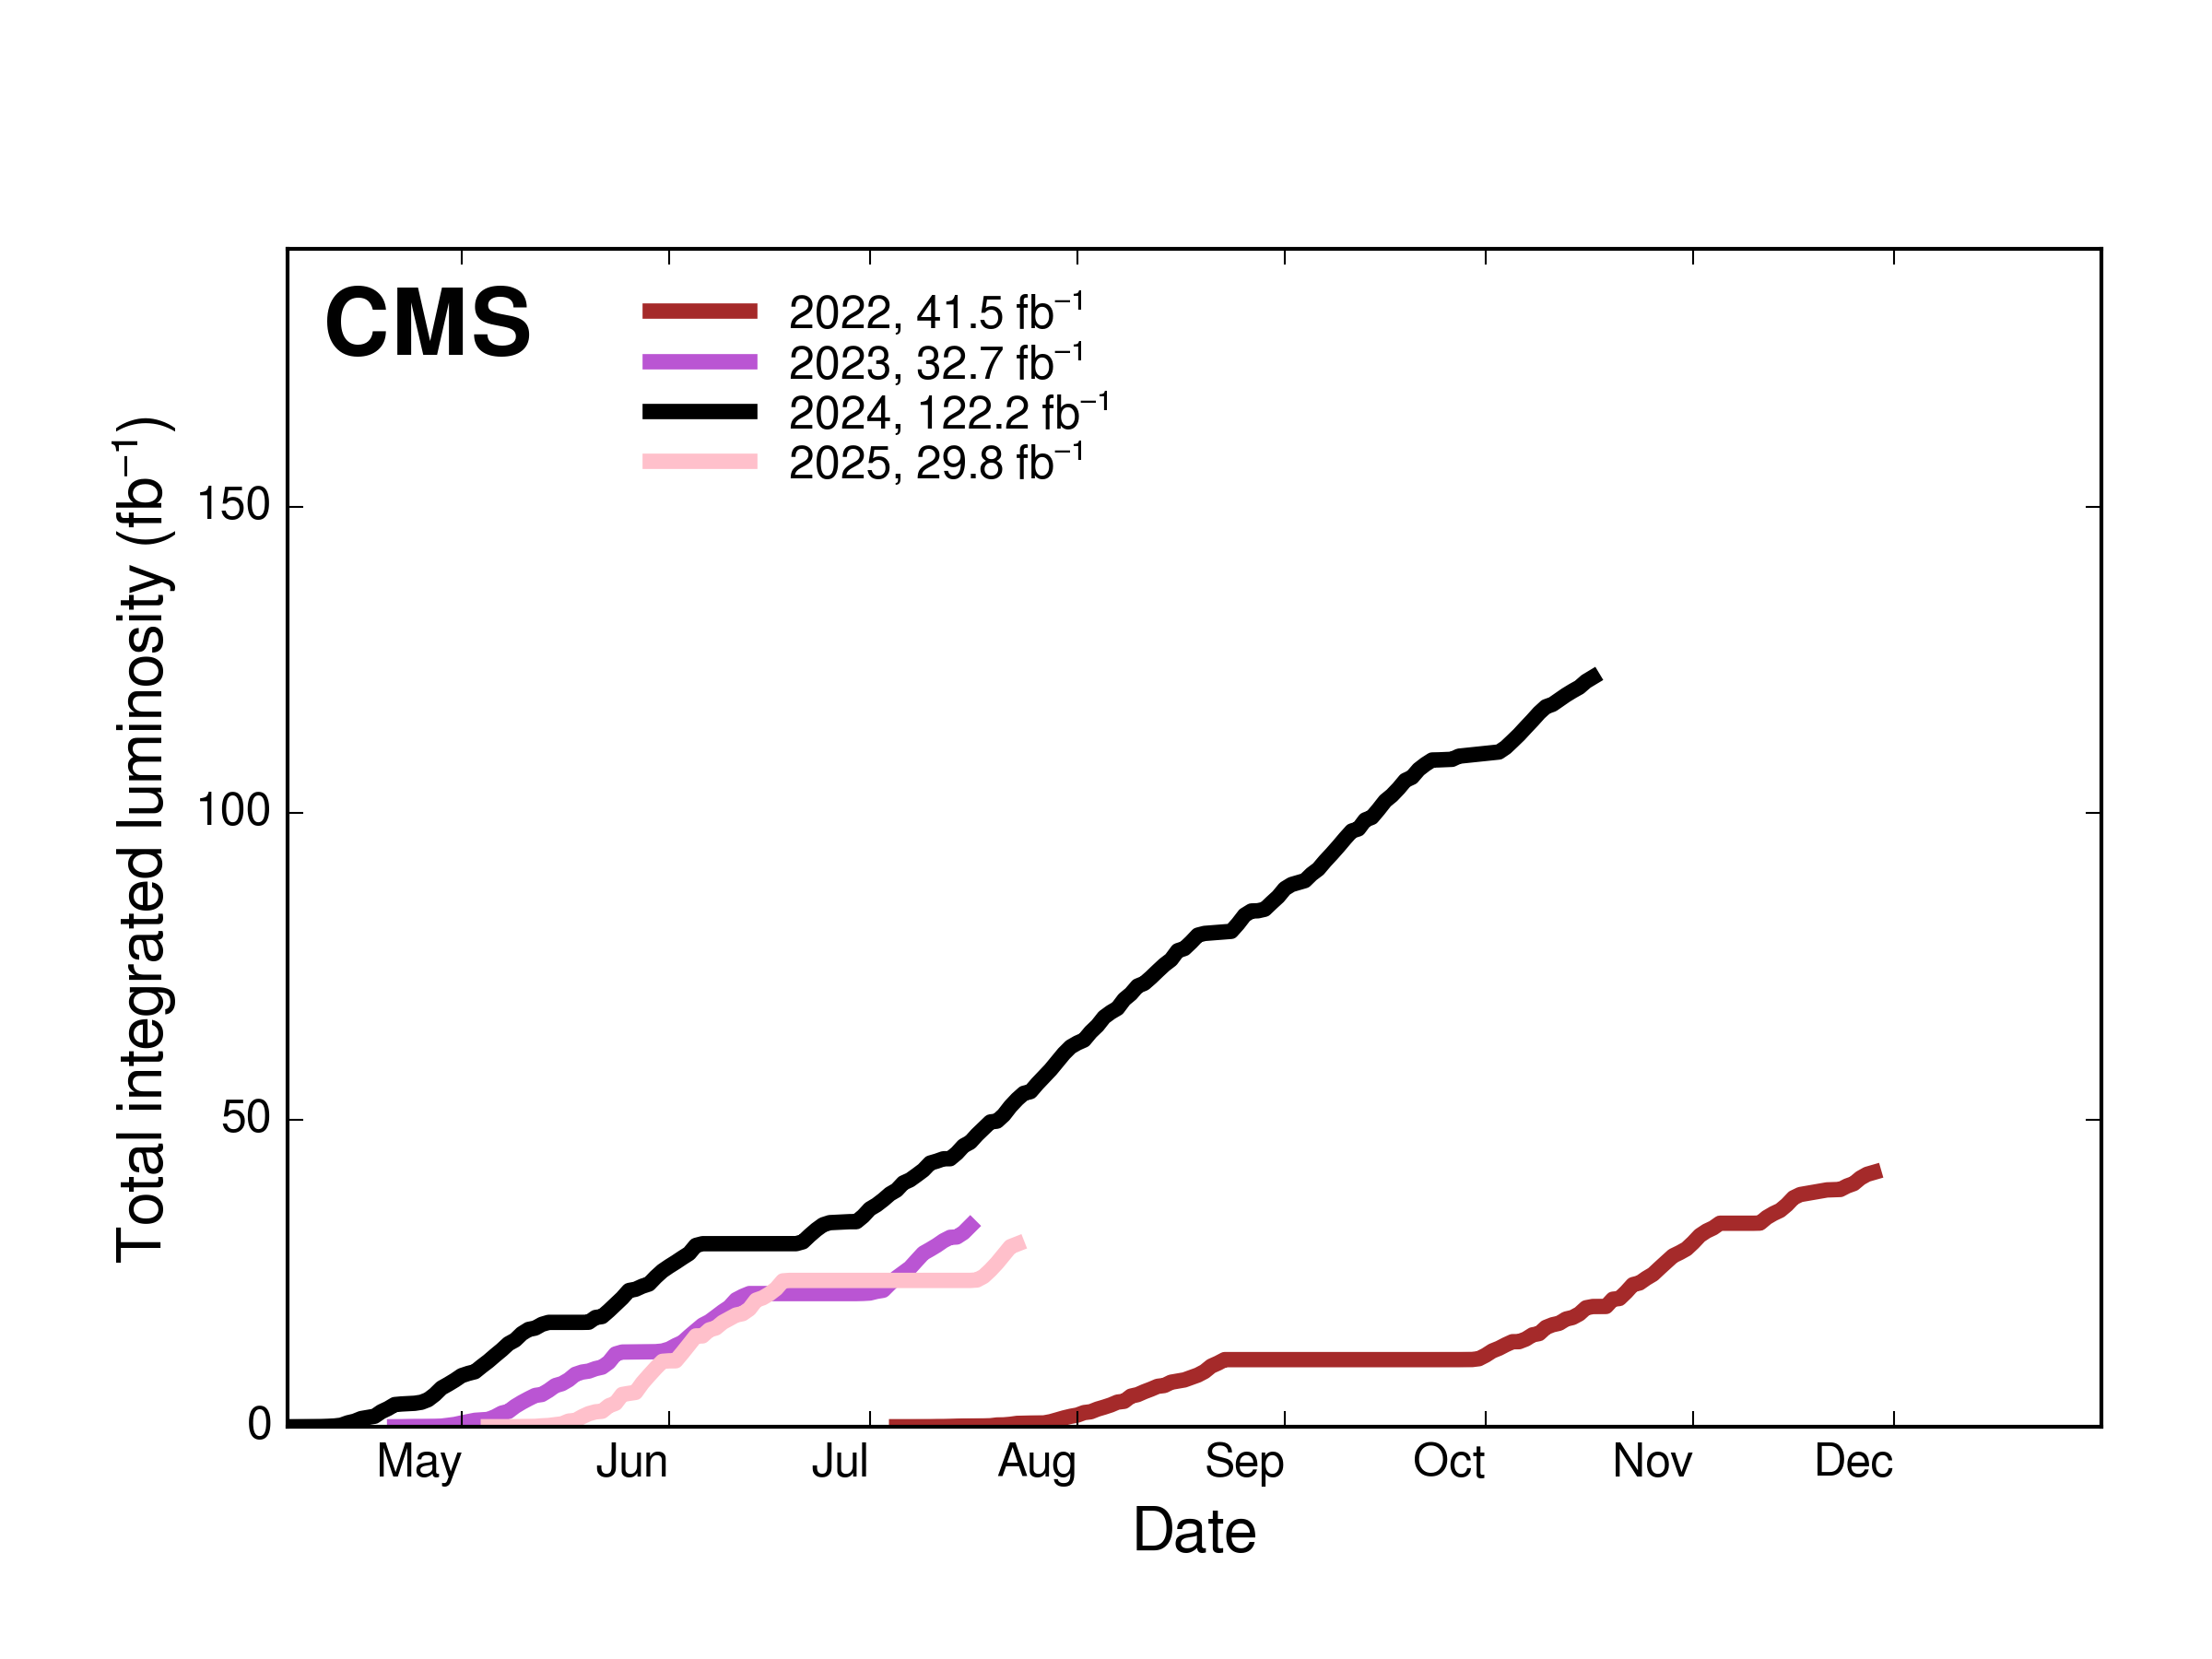
\includegraphics[width=0.82\linewidth]{figures/chap03-experiment-dataset/CMS_int_lumi_Run3.png}
  \caption{LHC 质子--质子对撞在 $\sqrt{s}=13.6$~TeV 下 CMS 接收的累计积分亮度与对撞机提供的积分亮度。提供的亮度对应于 CMS 前向强子量能器和像素探测器在数据质量筛选前测量的亮度，而记录的亮度要求所有 CMS 子探测器处于运行状态。\cite{CMS:LUMI-PUB}。}
  \label{fig:chap03-luminosity-run3}
\end{figure}

\begin{figure}
  \centering
  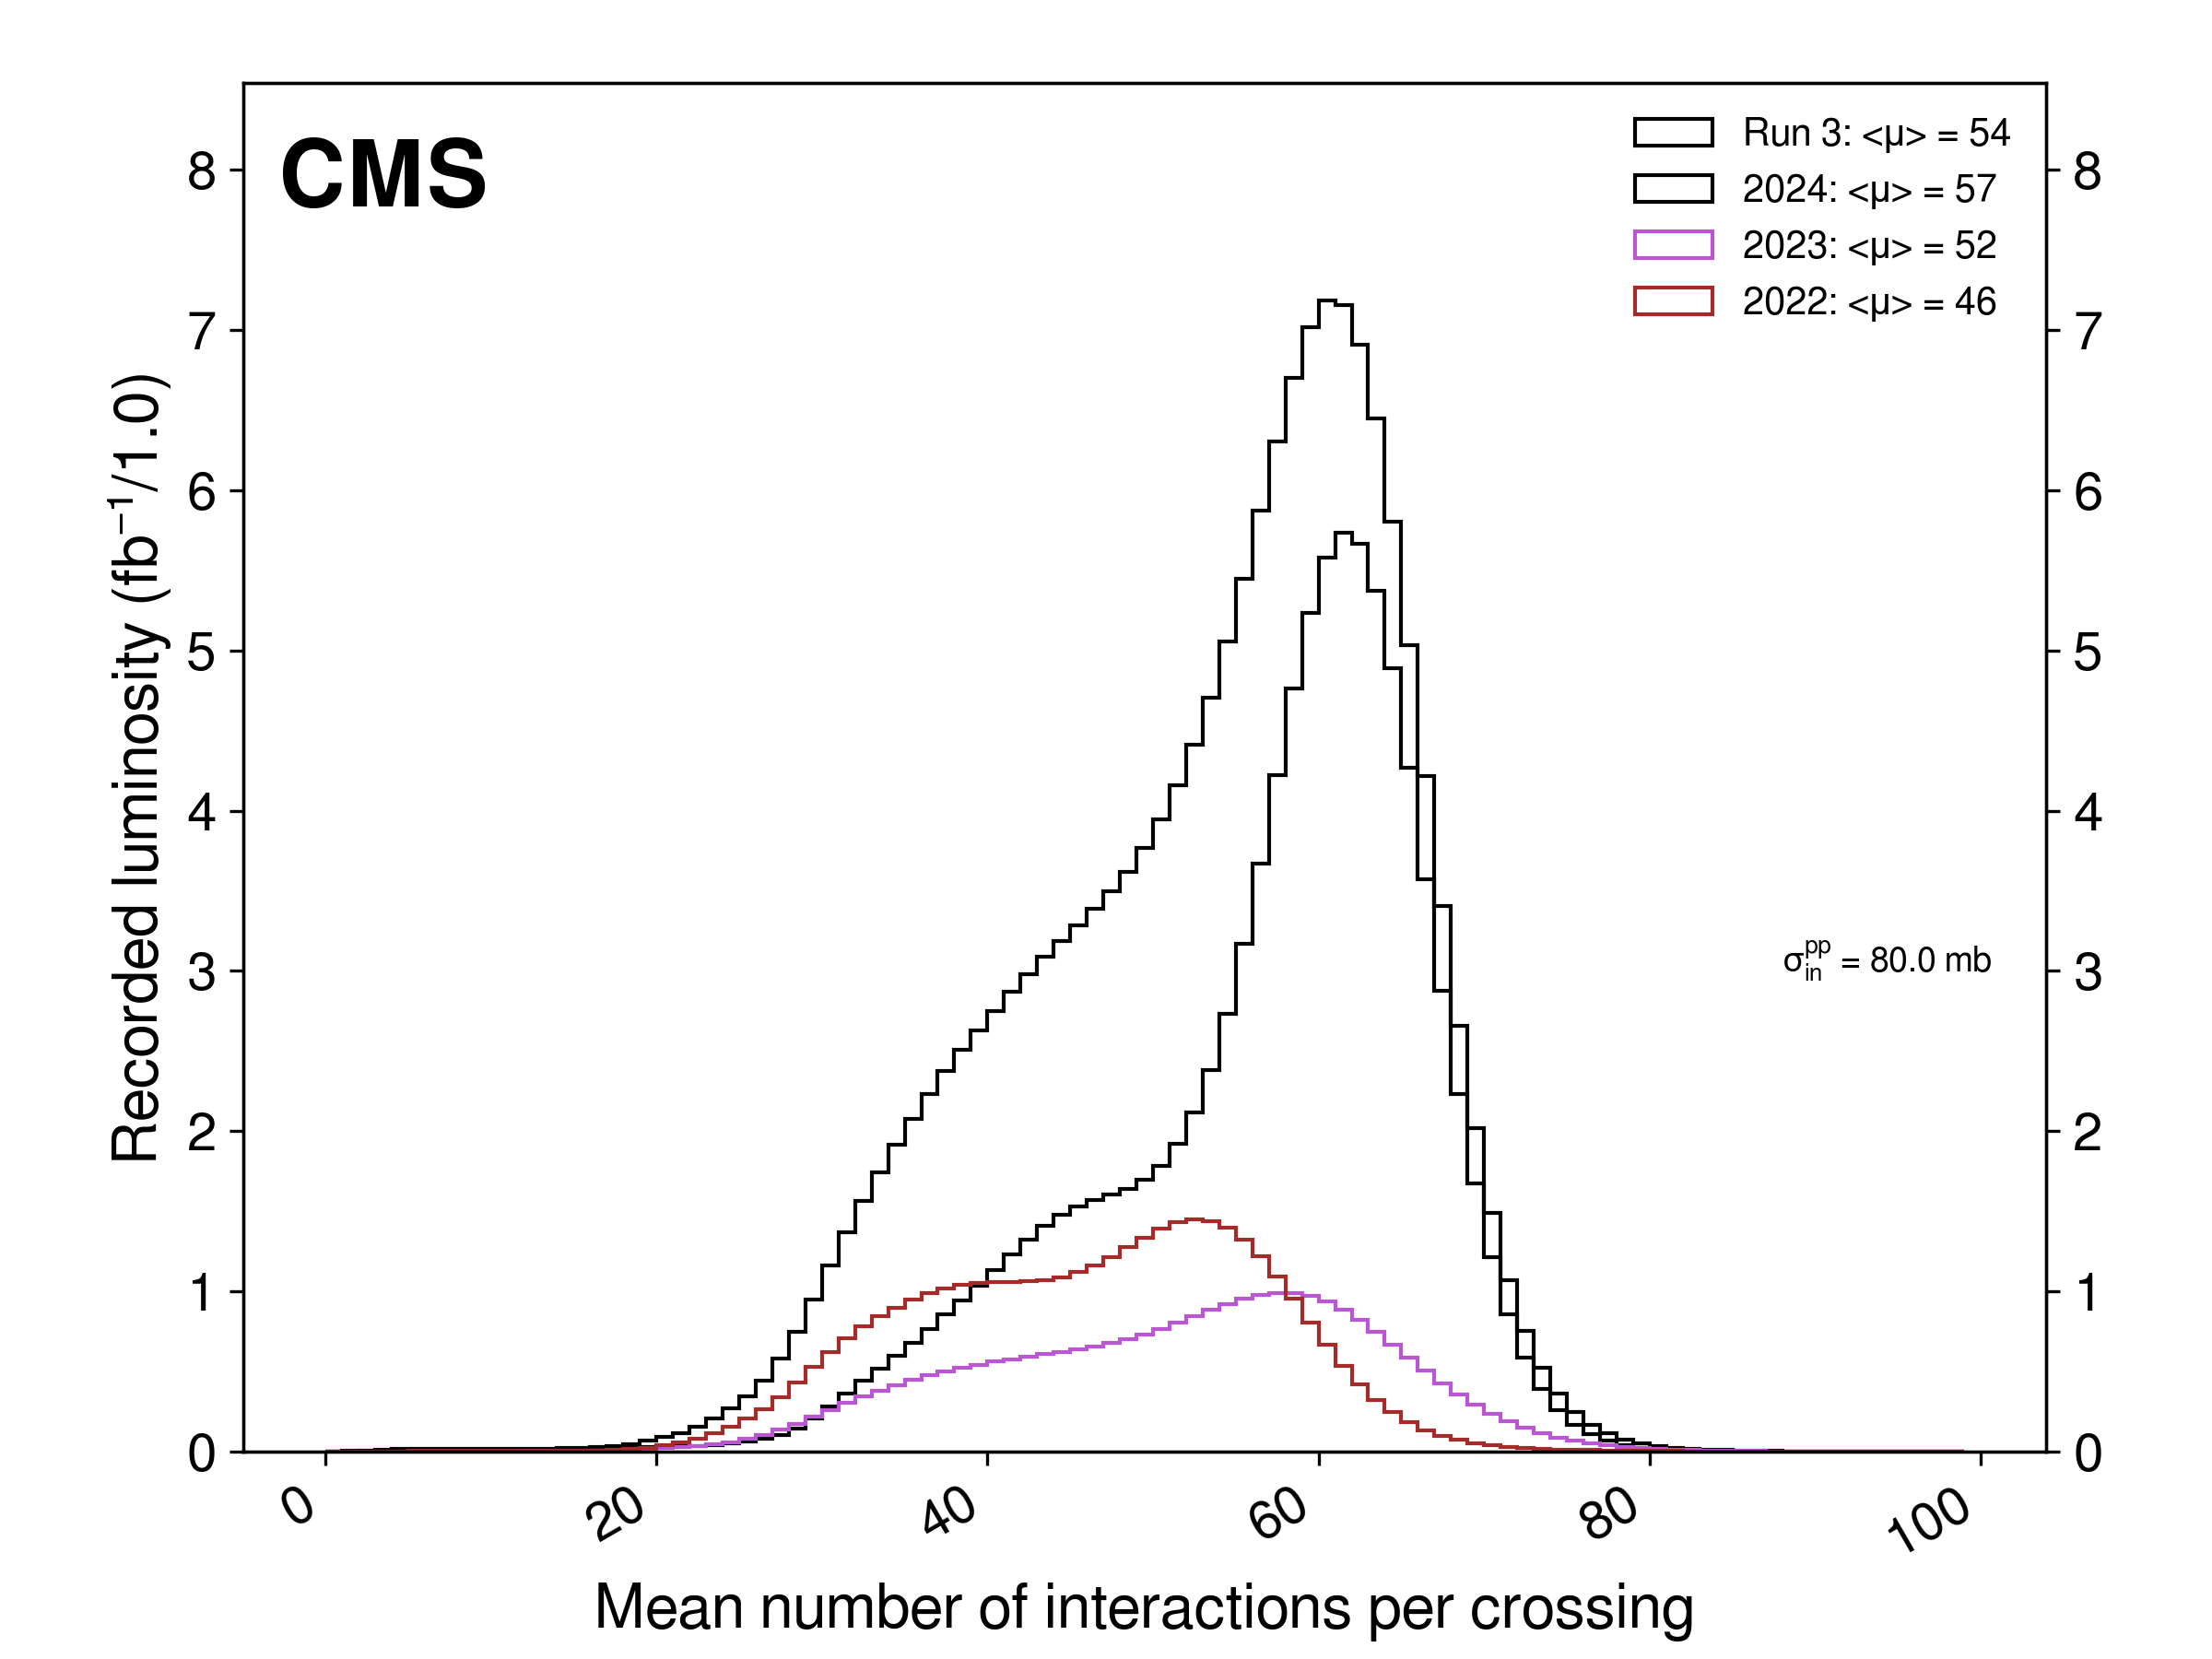
\includegraphics[width=0.82\linewidth]{figures/chap03-experiment-dataset/CMS_pileup_allYears_run3.png}
  \caption{在认证为物理分析可用的数据采集期间，CMS 每次束团交叉中质子--质子相互作用平均数（堆叠）的分布。该分布反映了 LHC 的高亮度运行条件。\cite{CMS:LUMI-PUB}。}
  \label{fig:chap03-pileup-run3}
\end{figure}

\section{模拟样本}
% \section{Simulation Samples}

% [PENDING]
蒙特卡罗（Monte Carlo, MC）模拟样本用于估计几何接收度、触发和重建效率、选择效率以及相关系统误差。模拟链包含以下环节：硬散射事例产生、部分子簇射和强子化、探测器响应模拟、数字化与堆叠混合、触发模拟，以及基于 CMSSW 的离线重建。粒子流重建在 CMS 事件描述中综合使用径迹、量能器和缪子系统信息~\cite{CMS_PF_RECO_JINST_2017}，但本分析对最终重建对象的使用方式在第 4 章中定义。各环节的关键配置如下。

\subsection{信号过程与产生子配置}

$pp \to J/\psi + J/\psi + \phi + X$ 的产生机制包括单部分子散射（SPS）、双部分子散射（DPS）和三部分子散射（TPS）。SPS 过程包括 $gg \to c\bar{c}(^{3}S_{1}^{[1]}) + c\bar{c}(^{3}S_{1}^{[1]})$（LO 阶 $J/\psi+J/\psi$ 色单态产生，记为 SPS\_CS）及其伴随胶子辐射过程 $gg \to c\bar{c}(^{3}S_{1}^{[1]}) + c\bar{c}(^{3}S_{1}^{[1]}) + g$（NLO* 阶，记为 SPS\_G）。DPS 通过独立部分子散射事例的混合构建，分为两种拓扑：DPS1 混合两个 $gg \to J/\psi + g$（色单态与色八重态叠加）过程；DPS2\_CS 混合 $gg \to J/\psi+J/\psi$（LO 阶）与 $gg \to gg$（随后由部分子簇射产生 $\phi$），DPS2\_G 混合 $gg \to J/\psi+J/\psi+g$（NLO* 阶，含额外胶子辐射）与 $gg \to gg$（随后由部分子簇射产生 $\phi$）。LO 与 NLO* 矩阵元的区分由 \texttt{Helac-Onia} 自动处理~\cite{HS_SHAO_HO,HS_SHAO_HO_2}。在双 $J/\psi$ 产生的理论计算中，NLO* 实辐射修正（$\alpha_s^5$ 阶）对 $p_{\mathrm{T}}^{J/\psi} \gtrsim 5~\mathrm{GeV}$ 区域的贡献不可忽略~\cite{Lansberg:2014swa,Likhoded:2016}，这正是本分析增加 NLO* 样本的物理动机。应注意，$\phi$ 介子不一定需要在矩阵元层面显式包含末态胶子才能产生：$\phi$ 也可由初态或末态胶子的 backward shower 碎裂得到，因此本分析的 SPS\_CS 和 SPS\_G 过程均被保留。TPS 混合两个 $gg \to J/\psi + g$ 与一个 $gg \to gg$（随后由部分子簇射产生 $\phi$）；各产生机制的相对贡献由后续截面测量或唯象拟合确定。\textbf{[注意：TPS 样本尚未完成产生。]}

硬散射事例使用 \texttt{Helac-Onia}~2.7.6~\cite{HS_SHAO_HO} 进行矩阵元计算并输出 \textsc{Les Houches} 事件文件（LHE）。采用 PHEGAS 蒙特卡洛积分器，部分子分布函数选用 CTEQ6M。色八重态长程矩阵元（LDME）取自邵华圣和张玉杰 $J/\psi+\Upsilon$ 联合产生分析的 Set~3~\cite{Shao:2016:JpsiUpsilon}。

\subsection{部分子簇射、强子化与 \texorpdfstring{\(\phi\)}{phi} 产生}

使用独立编译的 \textsc{Pythia}~8 进行部分子簇射和强子化~\cite{PYTHIA_8_2}，通过 \textsc{HepMC3} 接口输出事例记录。采用 CMS Run~3 对应的 CP5 调谐参数（$\text{Tune:pp} = 14$），PDF 选用 NNPDF3.1 NNLO（$\alpha_{s}(M_{Z}) = 0.118$）。对于色八重态夸克偶素，设置 $\texttt{OniaShower:octetSplit} = 1$（允许色八重态通过辐射软胶子并演化至色单态）和 $\texttt{Onia:massSplit} = 0.2$，后者是色八重态经簇射演化至最终色中性夸克偶素束缚态的必要配置。$J/\psi$ 强制衰变到 $\mu^{+}\mu^{-}$ 对，$\phi$ 强制衰变到 $K^{+}K^{-}$ 对。

目前尚无专门针对 $\phi$ 介子的矩阵元产生子能够在硬散射层面可靠地产生 $\phi$。因此，本分析中 $\phi$ 介子的产生未在矩阵元层面处理，而是通过 $gg \to gg$ 过程在部分子层次产生胶子对，再由 \textsc{Pythia}~8 的部分子簇射和强子化将末态胶子碎裂为 $\phi$ 介子。$\phi$ 介子通过软 QCD 过程大量产生，而在硬散射中产生率相对较低。为在模拟中获得足够的 $\phi$ 介子统计量，含 $\phi$ 的末态过程采用增强模式：关闭 \textsc{Pythia}~8 的多重部分子相互作用（MPI），在完成部分子层次计算后保存状态，通过循环调用 $\texttt{forceHadronLevel}$ 直至强子化末态中出现满足 $p_{\mathrm{T}} > 3.0~\mathrm{GeV}$ 的 $\phi$ 介子。需注意，此方法通过反复尝试强子化来增强特定末态粒子的产额，可能引入选择偏差——这是当前模拟方案的一个已知局限。对于仅需识别 SPS 中 $\phi$ 产生来源的情形，关闭 MPI 后直接将标准 \textsc{Pythia}~8 簇射输出接至 $\phi$ 寻找，不启用增强循环，可提供无偏差的参照。$\phi$ 的 $p_T$ 谱在数据与 MC 之间存在一定差异（尤其 $p_T > 10~\mathrm{GeV}$ 区域 MC 偏软），这是胶子碎裂模型固有的局限，将在系统误差中予以考虑。

\subsection{事例混合与 TPS 模拟}

\textsc{Pythia}~8 无法原生处理三个独立硬散射过程的同时部分子簇射和强子化。标准的 \textsc{Pythia}~8 框架仅支持单次硬散射的簇射演化，而对于 DPS 或 TPS 中并发的多个硬散射，缺乏描述它们之间量子干涉、色关联和动量共享的完备模型。因此，本分析的 DPS 和 TPS 模拟未在 \textsc{Pythia}~8 中直接生成，而是采用事例混合方案：首先独立产生各个 SPS 事例并分别通过 \textsc{Pythia}~8 进行簇射和强子化，再根据 DPS 或 TPS 拓扑将对应个数的 \textsc{HepMC} 事例合并为一个复合事例。各输入文件按事件数对齐至最少者，合并后的事例再送入 \textsc{CMSSW} 进行探测器模拟和重建。

\subsection{探测器模拟与重建}

基于 \textsc{Geant4} 的 CMS 探测器模拟~\cite{GEANT4}，模拟框架为 \textsc{CMSSW\_12\_4\_14}。采用扩展几何描述（$\texttt{DB:Extended}$），全局标签为 $124\mathrm{X}\_\mathrm{mcRun3\_2022\_realistic\_v12}$，对撞束斑设置为 $13.6~\mathrm{TeV}$ 的 2022 年早期条件，HLT 菜单为 2022v12。堆叠采用 Run~3 2022 夏季预混合样本（$\texttt{Run3Summer22DRPremix}$），通过 CVMFS 上的预混合文件列表读取，数字化（DIGI）与数据混合（DATAMIX）后执行 L1 触发和 HLT。完整链路输出格式为 $\texttt{GEN-SIM} \to \texttt{RAW} \to \texttt{AODSIM} \to \texttt{MINIAODSIM}$。分析级 ntuple 使用 \textsc{CMSSW\_15\_0\_15} 及定制化的 NtupleMaker 软件包（$\texttt{TPS\_Onia2MuMu}$）从 $\texttt{MINIAODSIM}$ 产生，分析模式为 $\texttt{JpsiJpsiPhi}$。

\subsection{样本产生状态}

各产生机制对应的 MC 样本（campaign）产生状态如下。已完成且具有足够统计量的样本包括：DPS1（DPS1 拓扑）、DPS2\_CS（LO 阶 $J/\psi+J/\psi$ + $gg \to gg$，簇射产生 $\phi$）和 SPS\_CS（LO 阶 $J/\psi+J/\psi$ 色单态产生）。DPS2\_G（NLO* 阶，含额外胶子辐射）和 SPS\_G（NLO* 阶）样本已完成产生但统计量显著偏低：这是预期的，因为高阶硬散射过程涉及更复杂的矩阵元结构和更大的末态相空间，导致 \texttt{Helac-Onia} 积分收敛缓慢，单位计算时间的事例产额远低于对应的 LO 过程。TPS 样本（TPS）以及含 $\Upsilon$ 的相关样本（JUP 系列）尚未完成产生。

\begin{figure}
  \centering
  \fbox{\parbox{0.86\linewidth}{\centering
    \vspace{0.8cm}
    \textbf{MC 产生流程示意图}\\[6pt]
    \small
    $\underbrace{\texttt{Helac-Onia}~2.7.6}_{\text{硬散射矩阵元}}\;
    \xrightarrow{\text{LHE}}\;
    \underbrace{\textsc{Pythia}~8\;\;(\text{CP5, NNPDF3.1})}_{\text{簇射/强子化}}\;
    \xrightarrow{\text{HepMC}}\;
    \underbrace{\text{事例混合}}_{\text{DPS/TPS}}\;
    \xrightarrow{\text{HepMC}}\;
    \underbrace{\textsc{CMSSW\_12\_4\_14}}_{\text{探测器模拟}}\;
    \xrightarrow{\text{GEN-SIM}}\;
    \underbrace{\textsc{CMSSW\_12\_4\_14}}_{\text{数字化/堆叠/触发}}\;
    \xrightarrow{\text{RAW}}\;
    \underbrace{\textsc{CMSSW\_12\_4\_14}}_{\text{重建}}\;
    \xrightarrow{\text{AOD/MiniAOD}}\;
    \underbrace{\textsc{CMSSW\_15\_0\_15}}_{\text{分析 ntuple}}$\\[8pt]
    \normalsize
    条件：$124\mathrm{X}\_\mathrm{mcRun3\_2022\_realistic\_v12}$\quad
    HLT：2022v12\quad 束斑：Run~3 $13.6\ \mathrm{TeV}$ 早期\\[4pt]
    堆叠：$\texttt{Run3Summer22DRPremix}$（预混合）
    \vspace{0.8cm}
  }}
  \caption{信号和辅助 MC 样本的模拟产生流程。最终数据集标识符和 CMS 数据集路径将在 MC 生产完成后补充。}
  \label{fig:chap03-mc-flow}
\end{figure}

综上，本章介绍了LHC和CMS探测器的关键子系统——特别是硅径迹探测器、缪子系统和触发系统——以及本分析使用的$289.21~\mathrm{fb}^{-1}$ Run~3数据和MC模拟样本框架。基于这些实验条件，第4章将详细讨论从初级顶点重建到$J/\psi J/\psi\phi$候选筛选的完整分析链。
